% !TEX encoding = UTF-8
% !TEX TS-program = pdflatex
% !TEX root = ../tesi.tex

%**************************************************************
\chapter{Codifica}
\label{cap:codifica}
%**************************************************************
Dopo aver analizzato l'architettura del modulo \gls{ITF} insieme ai design pattern necessari alla realizzazione del prodotto passiamo ad analizzare nel dettaglio la struttura delle singole componenti.\\
I seguenti paragrafi analizzano quali metodi, attributi ed eventuali sottoclassi compongono i package più importanti necessari per la realizzazione del sistema.\\
Andremo ad analizzare:
\begin{itemize}
	\item \textbf{Data\_Identity\_Wallet} contenuto nel package \textit{Identity Wallet Handler};
	\item \textbf{Trusted Third Party} contenuto nel package \textit{Trusted Third Party Handler};
	\item \textbf{Data\_ID\_List} contenuto nel package \textit{ID List};
	\item \textbf{Data\_Identity} contenuto nel package \textit{Identity};
	\item \textbf{Personally Identifiable Information};
	\item \textbf{Key\_List} contenuto nel package \textit{TTP Key List};
	\item \textbf{Data\_Service\_Provider}contenuto nel package \textit{Service Provider Handler}.
\end{itemize}
\newpage
\section{Identity Wallet Handler}
\subsection{Data\_Identity\_Wallet}
\begin{figure}[h]
	\centering
	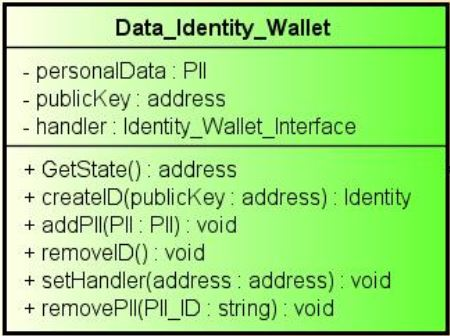
\includegraphics[width=0.5\textwidth]{immagini/identitywalletdata}
	\caption{Schema Data Identity Wallet}
\end{figure}
\begin{itemize}
	\item \textbf{Descrizione}\\
	Classe concreta utilizzata per modellare tutte le operazioni che un utente può effettuare con il sistema \gls{ITF}.
	\item \textbf{Attributi}
	\begin{itemize}
		\item \textit{- personalData: PII}\\
		Contiene le \gls{PII} che un utente ha inserito tramite l'applicativo e che vuole inserire nel proprio profilo;
		\item \textit{- publicKey: address}\\
		Chiave pubblica univoca che rappresenta l'identità di un utente all'interno del sistema \gls{ITF};
		\item \textit{- handler: Identity\_Wallet\_Interface}\\
		Oggetto necessario per l'implementazione del pattern \textit{strategy}. Tramite questo oggetto verranno invocati i metodi del modulo.
	\end{itemize}
	\item \textbf{Metodi}
	\begin{itemize}
		\item \textit{+ GetState(): void}\\
		Metodo necessario per realizzare il pattern \textit{observer} per la certificazione automatica delle \gls{PII}.
		\item \textit{+ createID(publicKey: address): identity}\\
		Metodo che permette la creazione di una nuova identità digitale all'interno del modulo \gls{ITF}.
		\textbf{Parametri:}
		\begin{itemize}
			\item \textit{publicKey: address}\\
			Chiave pubblica dell'identità che si vuole creare. Questo parametro è necessario per permettere l'associazione \textit{publicKey - indirizzo} in modo da andare a recuperare l'identità a partire dalla chiave pubblica.
		\end{itemize}
		\item \textit{+ addPII(PII: PII): void}\\
		Metodo necessario per aggiungere una o più nuove informazioni personali all'identità utente.\\\\
		\textbf{Parametri:}
		\begin{itemize}
			\item \textit{PII: PII}\\
			Informazioni personali che l'utente vuole inserire all'interno della propria identità digitale.
		\end{itemize}
		\item \textit{+ removeID(): void}\\
		Metodo che rimuove l'identità digitale dell'utente del sistema andando a cancellare la sua entry nella struttura dati che associa le chiavi pubbliche agli indirizzi delle identità.
		\item \textit{+ setHandler(address: address): void}\\
		Metodo necessario per impostare l'indirizzo dell'oggetto che deve andare ad implementare i metodi. Il metodo è segnato come pubblico anche se, grazie a \textit{Solidity}, bisogna impostare la proprietà dell'oggetto in modo che solo il proprietario del contratto possa cambiare l'indirizzo dell'oggetto che risolve i metodi.\\\\
		\textbf{Parametri:}
		\begin{itemize}
			\item \textit{address: address}
			Indirizzo dell'oggetto delegato alla risoluzione dei metodi.
		\end{itemize}
		\item \textit{+ removePII(PII\_ID: string): void}\\
		Metodo che permette ad un utente di rimuovere una o più informazioni personali che sono state inserite e certificate all'interno della propria identità digitale.\\\\
		\textbf{Parametri:}
		\begin{itemize}
			\item \textit{PII\_ID: string}\\
			Rappresenta l'identificativo univoco che va ad identificare l'informazione personale che si desidera rimuovere.
		\end{itemize}
	\end{itemize}
\end{itemize}
\section{Trusted Third Party Handler}
\subsection{Trusted Third Party}
\begin{figure}[!h]
	\centering
	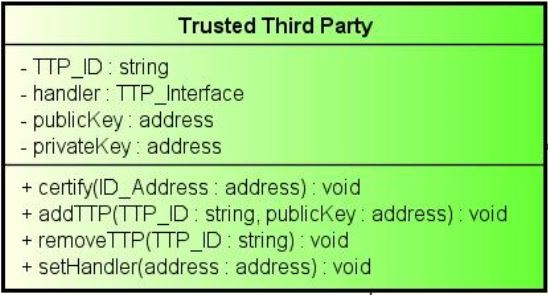
\includegraphics[width=0.5\textwidth]{immagini/ttpData}
	\caption{Schema Trusted Third Party}
\end{figure}
\begin{itemize}
	\item \textbf{Descrizione}\\
	Classe concreta utilizzata per modellare tutte le operazioni che un ente certificatore può fare sulle \gls{PII} di un utente ogni qual volta queste vengono aggiunte.\\
	Son presenti anche funzionalità per aggiungere e rimuovere nuovi enti certificatori.
	\item \textbf{Attributi}
	\begin{itemize}
		\item \textit{- TT\_ID: string}\\
		Rappresenta l'identificativo univoco mnemonico che identifica un ente certificatore.
		\item \textit{- handler: TTP\_Interface}\\
		Indirizzo dell'oggetto concreto che va a realizzare i metodi della classe, ponendo quindi fine alla catena di deleghe.
		\item \textit{- publicKey: address}\\
		Chiave pubblica utilizzata per permettere la decodifica, da parte del Service Provider Handler, del \textit{hash} per permettere la verifica.
		\item \textit{- privateKey: address}\\
		Chiave privata dell'ente certificatore necessaria per andare a certificare le informazioni personali dell'utente.
	\end{itemize}
	\item \textbf{Metodi}
	\begin{itemize}
		\item \textit{+ certify(ID\_Address: address): void}\\
		Metodo principale della classe Trusted Third Party. Compie la funzione, fondamentale, di andare a certificare le informazioni personali che un utente inserisce all'interno della sua identità digitale. Questa azione viene scatenata in automatico quando un utente aggiorna o inserisce nuove \gls{PII} grazie al pattern \textit{observer}.\\\\
		\textbf{Parametri:}
		\begin{itemize}
			\item \textit{ID\_Address: address}\\
			Indirizzo dell'oggetto Identity che rappresenta l'identità dell'utente che ha aggiunto una nuova \gls{PII}. Questo indirizzo è necessario per poter recuperare le informazioni personali aggiunte e per poterle certificare.			
		\end{itemize}
		\item \textit{+ addTTP(TTP\_ID: string, publicKey: address): void}\\
		Metodo che permettere di aggiungere un nuovo ente certificatore alla lista di enti che possono certificare le informazioni personali degli utenti. L'aggiunta avviene associando l'identificativo mnemonico con la chiave pubblica necessaria per l'attività di verifica delle informazioni certificate.\\\\
		\textbf{Parametri:}
		\begin{itemize}
			\item \textit{TTP\_ID: string}\\
			Identificativo univoco mnemonico che rappresenta un ente certificatore;
			\item \textit{publicKey: address}\\
			Chiave pubblica dell'ente certificatore necessaria per l'attività di verifica delle informazioni certificate.
		\end{itemize}
		\item \textit{+ removeTTP(TTP\_ID: string): void}\\
		Metodo necessario per poter rimuovere un ente certificatore dalla lista di quelli che possono certificare le informazioni degli utenti.\\\\
		\textbf{Parametri:}
		\begin{itemize}
			\item \textit{TTP\_ID: string}\\
			Identificativo univoco mnemonico necessario per specificare quale ente certificatore si vuole rimuovere dalla lista.
		\end{itemize}
		\item \textit{+ setHandler(address: address): void}\\
		Metodo necessario per impostare l'indirizzo dell'oggetto che deve andare ad implementare i metodi. Il metodo è segnato come pubblico anche se, grazie a \textit{Solidity}, bisogna impostare la proprietà dell'oggetto in modo che solo il proprietario del contratto possa cambiare l'indirizzo dell'oggetto che risolve i metodi.\\\\
		\textbf{Parametri:}
		\begin{itemize}
			\item \textit{address: address}\\
			Indirizzo dell'oggetto delegato alla risoluzione dei metodi.
		\end{itemize}
	\end{itemize}
\end{itemize}
\section{ID List}
\subsection{Data\_ID\_List}
\begin{figure}[!h]
	\centering
	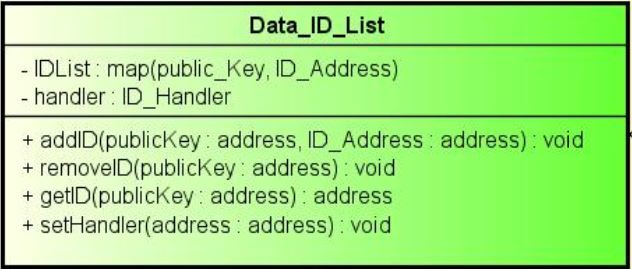
\includegraphics[width=0.5\textwidth]{immagini/dataIDList}
	\caption{Schema Data Identity List}
\end{figure}
\begin{itemize}
	\item \textbf{Descrizione}\\
	Classe concreta utilizzata per accoppiare l'identità di un utente (rappresentata dalla sua chiave pubblica) e le sue informazioni personali contenute nel proprio oggetto Identity.
	\item \textbf{Attributi}
	\begin{itemize}
		\item \textit{- IDList: map(publicKey, ID\_Address)}\\
		Componente fondamentale dell'intero package. Associa una chiave pubblica di tipo \textit{address} con l'indirizzo, sempre di tipo \textit{address}, associato all'oggetto identity che rappresenta le \gls{PII} dell'utente rappresentato dalla chiave pubblica inserita.\\
		Grazie a questa mappa è possibile, per ogni utente, recuperare le \gls{PII} a lui associate.
		\item \textit{- handler: ID\_Handler}\\
		Indirizzo dell'oggetto concreto che va a realizzare i metodi della classe, ponendo fine alla catena di deleghe.		
	\end{itemize}
	\item \textbf{Metodi}
	\begin{itemize}
		\item \textit{+ addID(publicKey: address, ID\_Address: address): void}\\
		Metodo che consente di aggiungere una nuova associazione utente-identità all'interno della mappa.\\\\
		\textbf{Parametri:}
		\begin{itemize}
			\item \textit{publicKey: address}\\
			Chiave pubblica associata all'utente che rappresenta il suo identificativo univoco;
			\item \textit{ID\_Address: address}\\
			Indirizzo \textit{Ethereum} che rappresenta un "puntatore" grazie al quale è possibile recuperare le \gls{PII} di un utente.
		\end{itemize}
		\item \textit{+ removeID(publicKey: address): void}\\
		Metodo che consente di rimuovere dalla mappa un'associazione utente-identità. In questo modo è possibile rendere irrecuperabile tutte le informazioni riguardanti un utente nel caso in cui questo decida di eliminare il proprio profilo dal sistema \gls{ITF}.\\\\
		\textbf{Parametri:}
		\begin{itemize}
			\item \textit{publicKey: address}\\
			Chiave pubblica (identificativo univoco) dell'utente della quale si vuole eliminare l'identità.
		\end{itemize}
		\item \textit{+ getID(publicKey: address): address}\\
		Metodo che consente di recuperare l'indirizzo dove trovare le informazioni personali dell'utente passato come parametro (tramite chiave pubblica).\\\\
		\textbf{Parametri:}
		\begin{itemize}
			\item \textit{publicKey: address}\\
			Chiave pubblica dell'utente della quale si vogliono recuperare le \gls{PII} per andare a verificare le sue informazioni.
		\end{itemize}
		\item \textit{+ setHandler(address: address): void}\\
		Metodo necessario per impostare l'indirizzo dell'oggetto che deve andare ad implementare i metodi. Il metodo è segnato come pubblico anche se, grazie a \textit{Solidity}, bisogna impostare la proprietà dell'oggetto in modo che solo il proprietario del contratto possa cambiare l'indirizzo dell'oggetto che risolve i metodi.\\\\
		\textbf{Parametri:}
		\begin{itemize}
			\item \textit{address: address}\\
			Indirizzo dell'oggetto delegato alla risoluzione dei metodi.
		\end{itemize}
	\end{itemize}
\end{itemize}
\newpage
\section{Identity}
\subsection{Data\_Identity}
\begin{figure}[!h]
	\centering
	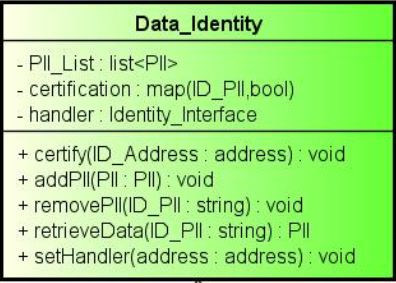
\includegraphics[width=0.5\textwidth]{immagini/identityData}
	\caption{Schema Data Identity}
\end{figure}
\begin{itemize}
	\item \textbf{Descrizione}\\
	Classe concreta utilizzata all'interno del sistema \gls{ITF} per rappresentare e manipolare l'identità di un utente.
	\item \textbf{Attributi}
	\begin{itemize}
		\item \textit{- PII\_List: list<PII>}\\
		Lista che contiene tutte le informazioni personali certificate associate ad un utente.
		\item \textit{- certification: map<ID\_PII. bool>}\\
		Mappa che, per ogni \gls{PII} presente nella lista, tiene traccia di quali sono certificate e quali no.
		\item \textit{- handler: Identity\_Interface}\\
		Indirizzo dell'oggetto concreto che va a realizzare i metodi della classe, ponendo quindi fine alla catena di deleghe.
	\end{itemize}
	\item \textbf{Metodi}
	\begin{itemize}
		\item \textit{+certify(ID\_Address: address): void}\\
		Metodo necessario all'ente certificatore per poter certificare tutte le informazioni personali che l'utente inserisce.\\\\
		\textbf{Parametri:}
		\begin{itemize}
			\item \textit{ID\_Address: address}\\
			Indirizzo delle informazioni personali da certificare.
		\end{itemize}
		\item \textit{+ addPII(PII: PII): void}\\
		Metodo utilizzato per aggiungere un'informazione personale all'interno della lista delle \gls{PII} associate all'utente.\\\\
		\textbf{Parametri:}
		\begin{itemize}
			\item \textit{PII: PII}\\
			Oggetto che rappresenta l'informazione personale che si vuole inserire e associare all'utente.
		\end{itemize}
		\item \textit{+ removePII(ID\_PII: string): void}\\
		Rimuove un'informazione personale dalla lista delle \gls{PII} associate all'utente.\\\\
		\textbf{Parametri:}
		\begin{itemize}
			\item \textit{ID\_PII: string}\\
			Identificativo univoco per identificare quale delle informazioni personali dell'utente si vuole rimuovere dalla sua lista.
		\end{itemize}
		\item \textit{+ retrieveData(ID\_PII: string): PII}\\
		Metodo utilizzato per recuperare tutto l'oggetto che rappresenta l'informazione personale dell'utente.\\\\
		\textbf{Parametri:}
		\begin{itemize}
			\item \textit{ID\_PII: string}\\
			Identificativo univoco mnemonico utilizzato per indicare quale delle informazioni personali recuperare dalla lista.
		\end{itemize}
		\item \textit{+ setHandler(address: address): void}\\
		Metodo necessario per impostare l'indirizzo dell'oggetto che deve andare ad implementare i metodi. Il metodo è segnato come pubblico anche se, grazie a \textit{Solidity}, bisogna impostare la proprietà dell'oggetto in modo che solo il proprietario del contratto possa cambiare l'indirizzo dell'oggetto che risolve i metodi.\\\\
		\textbf{Parametri:}
		\begin{itemize}
			\item \textit{address: address}\\
			Indirizzo dell'oggetto delegato alla risoluzione dei metodi.
		\end{itemize}
	\end{itemize}
\end{itemize}
\section{Personally Identifiable Information}
\begin{figure}[!h]
	\centering
	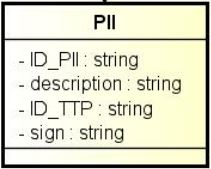
\includegraphics[width=0.5\textwidth]{immagini/pii}
	\caption{Schema Personally Identifiable Information}
\end{figure}
\begin{itemize}
	\item \textbf{Descrizione}\\
	Classe concreta necessaria che rappresenta un informazione personale dell'utente all'interno del sistema \gls{ITF}.
	\item \textbf{Attributi}\\
	\begin{itemize}
		\item \textit{- ID\_PII: string}\\
		Identificativo univoco mnemonico necessario per individuare facilmente la \gls{PII}.
		\item \textit{- description: string}\\
		Campo che descrive il tipo di informazione personale.
		\item \textit{- ID\_TTP: string}\\
		Identificativo univoco mnemonico che rappresenta l'ente certificatore che ha certificato, tramite firma, la \gls{PII}.
		\item \textit{- sign: string}\\
		Firma che certifica la \gls{PII}. Questa firma è ottenuta dall'\textit{hash} dei dati uniti alla chiave privata dell'ente certificatore che vuole certificarli.
	\end{itemize}
\end{itemize}
\section{TTP Key List}
\subsection{Key\_List}
\begin{figure}[!h]
	\centering
	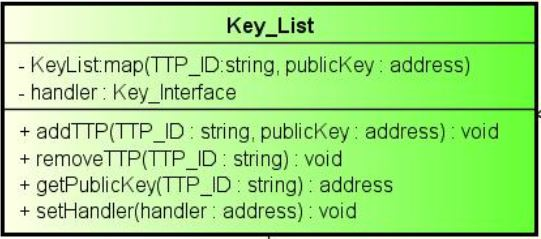
\includegraphics[width=0.5\textwidth]{immagini/keylistData}
	\caption{Schema Key List}
\end{figure}
\begin{itemize}
	\item \textbf{Descrizione}\\
	Classe concreta che mantiene una mappa che consente di associare un identificativo mnemonico, che rappresenta un ente certificatore, e la sua chiave pubblica necessaria per poter verificare le \gls{PII} certificate.
	\item \textbf{Attributi}
	\begin{itemize}
		\item \textit{- KeyList: map<TTP\_ID: string, publicKey: address>}\\
		Mappa che mantiene tutte le associazioni tra identificativo univoco mnemonico e rispettive chiavi pubbliche.\\
		Questa lista è necessaria per poter recuperare, dato l'ID della \gls{TTP}, la chiave pubblica per la successiva verifica delle informazioni personali dell'utente.
		\item \textit{- handler: key\_interface}\\
		Indirizzo dell'oggetto concreto che va a realizzare i metodi della classe, ponendo quindi fine alla catena di deleghe.		
	\end{itemize}
	\item \textbf{Metodi}
	\begin{itemize}
		\item \textit{+ addTTP(TTP\_ID: string, publicKey: address): void}\\
		Metodo pensato per poter espandere la lista di enti certificatori che possono certificare le informazioni personali contenute nel sistema.\\\\
		\textbf{Parametri:}
		\begin{itemize}
			\item \textit{TTP\_ID: string}\\
			Identificativo univoco mnemonico necessario per permettere l'associazione delle informazioni;
			\item \textit{publicKey: address}\\
			Chiave pubblica dell'ente certificatore che si desidera agiungere alla mappa.
		\end{itemize}
		\item \textit{+ removeTTP(TTP\_ID: string): void}\\
		Metodo che consente di rimuovere gli enti certificatori dalla lista di quelli idonei a certificare le \gls{PII} degli utenti.\\\\
		\textbf{Parametri:}
		\begin{itemize}
			\item \textit{TTP\_ID: string}\\
			Identificativo univoco mnemonico dell'ente certificatore che si desidera rimuovere dalla lista degli enti idonei alla certificazione.
		\end{itemize}
		\item \textit{+ getPublicKey(TTP\_ID: string): address}\\
		Metodo che consente di recuperare la chiave pubblica a partire dall'identificativo univoco mnemonico dell'ente certificatore.\\\\
		\textbf{Parametri:}
		\begin{itemize}
			\item \textit{TTP\_ID: string}\\
			Identificativo univoco mnemonico dell'ente certificatore della quale si desidera recuperare la chiave pubblica.
		\end{itemize}
		\item \textit{+ setHandler(address: address): void}\\
		Metodo necessario per impostare l'indirizzo dell'oggetto che deve andare ad implementare i metodi. Il metodo è segnato come pubblico anche se, grazie a \textit{Solidity}, bisogna impostare la proprietà dell'oggetto in modo che solo il proprietario del contratto possa cambiare l'indirizzo dell'oggetto che risolve i metodi.\\\\
		\textbf{Parametri:}
		\begin{itemize}
			\item \textit{address: address}\\
			Indirizzo dell'oggetto delegato alla risoluzione dei metodi.
		\end{itemize}
	\end{itemize}
\end{itemize}
\newpage
\section{Service Provider Handler}
\subsection{Data\_Service\_Provider}
\begin{figure}[!h]
	\centering
	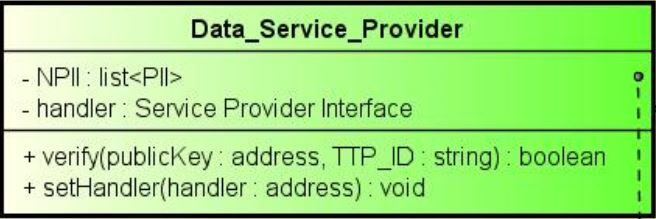
\includegraphics[width=0.5\textwidth]{immagini/dataSP}
	\caption{Schema Data Service Provider}
\end{figure}
\begin{itemize}
	\item \textbf{Descrizione}\\
	Classe concreta utilizzata per manipolare tutte le informazioni personali che il serivce provider deve verificare prima di permettere l'accesso e l'erogazione di servizi all'utente che li ha richiesti.
	\item \textbf{Attributi}
	\begin{itemize}
		\item \textit{- NPII: list<PII>}\\
		\textit{Not PII} nome dato alla lista delle \gls{PII} che il service provider richiede siano verificate per poter rilasciare il servizio all'utente che li ha richiesti.
		\item \textit{- handler: Service\_Provider\_Interface}\\
		Indirizzo dell'oggetto concreto che va a realizzare i metodi della classe ponendo fine alla catena di deleghe.
	\end{itemize}
	\item \textbf{Metodi}
	\begin{itemize}
		\item \textit{+ verify(publicKey: address, TTP\_ID:string): boolean}\\
		Metodo fondamentale del package che consente la verifica delle informazioni personali dell'utente passato come parametro (identificato tramite la sua chiave pubblica).\\
		Dalla chiave pubblica, utilizzando ID List, è possibile recuperare le \gls{PII} associate all'utente e verificare che siano certificate.\\
		La verifica avviene tramite confronto dell'\textit{hash} nel \gls{PII} con il nuovo \textit{hash} calcolato a partire dai dati e la chiave pubblica del \gls{TTP}.\\
		La chiave pubblica del \gls{TTP} viene recuperata tramite TTP\_ID utilizzando il package TTP Key List.\\\\
		\textbf{Parametri:}
		\begin{itemize}
			\item \textit{publicKey: address}\\
			Chiave pubblica necessaria per recuperare le \gls{PII} dell'utente che ha richiesto l'accesso ad un servizio;
			\item \textit{TTP\_ID: string}\\
			Identificativo univoco mnemonico dell'ente certificatore che ha certificato le informazioni personali. Questo attributo è utilizzato per recuperare la chiave pubblica necessaria per la verifica degli \textit{hash}.
		\end{itemize}
		\item \textit{+ setHandler(address: address): void}\\
		Metodo necessario per impostare l'indirizzo dell'oggetto che deve andare ad implementare i metodi. Il metodo è segnato come pubblico anche se, grazie a \textit{Solidity}, bisogna impostare la proprietà dell'oggetto in modo che solo il proprietario del contratto possa cambiare l'indirizzo dell'oggetto che risolve i metodi.\\\\
		\textbf{Parametri:}
		\begin{itemize}
			\item \textit{address: address}\\
			Indirizzo dell'oggetto delegato alla risoluzione dei metodi.
		\end{itemize}		
	\end{itemize}
\end{itemize}
